\definecolor{exxetagray}{gray}{0.75}
\definecolor{itemcolor}{RGB}{179,217,255}
\definecolor{usercolor}{RGB}{255,204,179}

\shorthandoff{"}
\chapter{Verwandte Arbeiten}
\label{ch:verwandte_arbeiten}
In der Literatur existieren bereits einige Arbeiten, die sich mit der Berücksichtigung wechselseitiger Präferenzen in der Empfehlungserstellung beschäftigen.
Auch der Bereich der multi-kriteriellen Empfehlungssysteme wurde in der Literatur in diversen Veröffentlichungen behandelt.
Nachfolgend werden verwandte Arbeiten zu reziproken Empfehlungssystemen sowie zu multi-kriteriellen Empfehlungssystemen mit Bezug auf die vorliegende Domäne angeführt.

\section{Reziproke Systeme}

\subsection{Systeme mit identischer Gewichtung der Präferenzen}
% d.h. wie sehr zwei personen übereinstimmen, beides gleich gewichtet
% Dual perspektive graph representation hier: S. 104, file://wsl%24/Ubuntu/home/masc6/Projects/masterarbeit/literatur/recsys%202022%20modeling%20two%20way%20selection%20preference%20for%20person%20job%20fit.pdf

\subsection{Systeme mit unterschiedlicher Gewichtung der Präferenzen}
% präferenz eines nutzers höher gewichtet als präferenz der empfohlenen Elemente
% feature optionen können 3 unterschiedliche stadi annehmen. -> classification (label mit match und kein match) S. 68, file://wsl%24/Ubuntu/home/masc6/Projects/masterarbeit/literatur/DiazMetzlerAmer-Yahia%20-%20Relevance%20and%20Ranking%20in%20Online%20Dating%20Systems%20(2010)%20-%200.pdf
% Johannes Thesis

\section{Multi-kriterielle Systeme}
hier bsp anführen für arbeiten die sich mit mk systemen beschäftigen in den 3 bereichen
% Hier erwähnen, dass nicht alle systeme auch als mk-systeme bezeichnet sind, die solche Ansätze anwenden (bspw. hybride systeme)
% Hier erwähnen, dass Fokus auf aggregation mehrerer Kriterien und deren gewichtung liegt -> hiernach suchen

% Verwendung von MAUT (siehe S. 432, file://wsl%24/Ubuntu/home/masc6/Projects/masterarbeit/literatur/Analysis%20and%20Classification%20of%20Multi-Criteria.pdf)
% MAUT in utility based recommenders: file://wsl%24/Ubuntu/home/masc6/Projects/masterarbeit/literatur/Designing%20utility-based%20recommender%20systems%20for%20e-commerce.pdf

\subsection{Multi-attribut basierte Systeme}
% hybrid recommender: weighted -> S. 339, https://link.springer.com/content/pdf/10.1023/A:1021240730564.pdf?pdf=button

\subsection{Multi-objektive Systeme}
% multi-objective example: S. 237, file://wsl%24/Ubuntu/home/masc6/Projects/masterarbeit/literatur/Adaptive%20multi%20attribute%20diversity%20for%20recommender%20systems.pdf

Als multi-objektiv bezeichnen \textcite[S. 12]{rodriguez:inproceedings} ihren Ansatz zur Integration "äußerer Merkmale"\footnote{"extraneous features" - \textcite[S. 12]{rodriguez:inproceedings}} in ein semantisches Modell im Bereich des Online-Recruitments. 
Dieser ist in Abbildung \ref{fig:relatedwork:abb1} dargestellt.

\begin{figure}
    \centering
	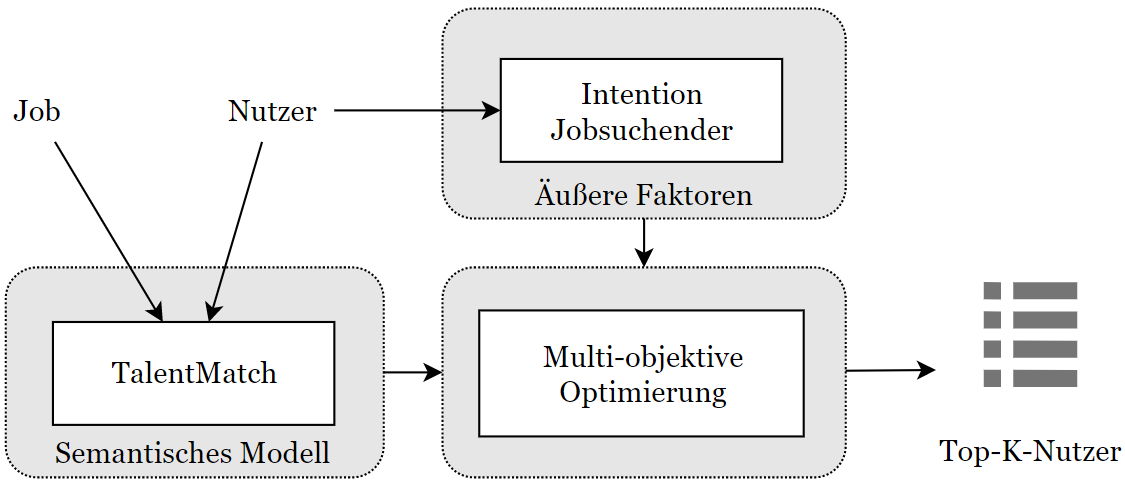
\includegraphics[width=0.9\textwidth]{gfx/talentMatch.png}
	\caption[Ansatz für die Integration äußerer Merkmale in semantische Modelle]{Ansatz für die Integration äußerer Merkmale in semantische Modelle\\
    (Eigene Darstellung in Anlehnung an \cite[S. 12]{rodriguez:inproceedings})}
	\label{fig:relatedwork:abb1}
\end{figure}

Im Detail stellen die Autoren eine Erweiterung des bestehenden \textit{TalentMatch}-Systems des sozialen Netzwerks LinkedIn vor, welche neben des semantischen Matches \cite[S. 2]{jannach:2:inproceedings} zwischen einer Person und einem Job (Objective 1) zusätzlich die Offenheit einer Person für Jobangebote (Objective 2) in die Empfehlungserstellung (Ranking) miteinbezieht.
Dabei gehen die Autoren davon aus, dass die beiden Ziele möglicherweise miteinander konkurrieren, d.h. dass eine Person, die am besten auf eine Jobbeschreibung zutrifft, möglicherweise nicht offen für eine neue Stelle ist.
\textcite[S. 12]{rodriguez:inproceedings} untersuchen in ihrer Arbeit, ob die Berücksichtigung der Neigung von Personen für offene Jobpositionen den Nutzen der Nutzer des Systems dennoch positiv beeinflusst.
Den Nutzen operationalisieren die Autoren als das Engagement zwischen Jobsuchenden und Anbietern von Jobpositionen \cite[S. 14]{rodriguez:inproceedings}, welche diese über Menge aktiver und passiver Nutzer in dem System messen.
Die Integration der Berücksichtigung in das semantische Modell führen \textcite[S. 15]{rodriguez:inproceedings} systematisch über ein Re-Ranking durch.
Dies realisieren \textcite[S. 13]{rodriguez:inproceedings} über folgende Verlust-Funktion $L$:
\begin{equation}\label{eq30}
    L(\alpha ,\beta) = -g(f(Y, X, [\alpha , \beta])) + \Delta (\pi (Y), \pi (f(Y,X,[\alpha ,\beta])))
\end{equation}
Nach \textcite[S. 13]{rodriguez:inproceedings} gibt $g$ die durchschnittliche Anzahl aktiver und passiver Nutzer in dem erweiterten System $f(Y, X, [\alpha , \beta])$ und $\Delta$ die Abweichung des Rankings $\pi (f(Y,X,[\alpha ,\beta]))$ des erweiterten Systems im Vergleich zu dem Ranking $\pi (Y)$ des ursprünglichen semantischen Modells an.
Die Anpassung eines semantischen Matches $y$ realisieren \textcite[S. 15]{rodriguez:inproceedings} durch einen sogenannten "Boost", wobei dieser für aktive ($\alpha$) und passive ($\beta$) Nutzer unterschieden werden kann:
\begin{equation}\label{eq31}
    f(y,x,[\alpha ,\beta]) = y \times (\alpha^{1\{{x == \textnormal{active}\}}}) \times (\beta^{1\{{x == \textnormal{active}\}}})
\end{equation}
Hierbei ist $1\{x == \textnormal{active}\}$ gleich $1$, wenn die Bedingung innerhalb der geschweiften Klammer wahr ist und $0$ andernfalls.
\textcite[S. ]{rodriguez:inproceedings}
% HIER WEITERMACHEN und ergebnisse anführen!
% Bis dato könnte dieser Ansatz unserer Idee am nächsten kommen

\subsection{Multi-kriterielle Bewertungen in Empfehlungssystemen}
% Erfinder des aggregation Funktion approaches: file://wsl%24/Ubuntu/home/masc6/Projects/masterarbeit/literatur/New_Recommendation_Techniques_for_Multicriteria_Rating_Systems.pdf
% Arbeit von Jannach wie hier beschrieben mit SVM: S. 102, file://wsl%24/Ubuntu/home/masc6/Projects/masterarbeit/literatur/E-Commerce.pdf
% multi-kriteria: Aggregation function approach: file://wsl%24/Ubuntu/home/masc6/Projects/masterarbeit/literatur/Recommending%20Hotels%20based%20on%20Multidimesional%20Customer%20Ratings.pdf
% ansatz von Tang: zusammenfügen mehrere feature bewertungen, sowie durchschnittsbewertung und kommentare, file:///C:/Users/masc6/Downloads/tdladmin,+TangandMcCalla_JoDI_final.pdf
% Slope one algorithmus und adaptive genetic algorithm von Hassan, S. 327, file://wsl%24/Ubuntu/home/masc6/Projects/masterarbeit/literatur/Imrpoving%20Prediction%20accuracy%20of%20multi-criteria%20recommender.pdf
% Liu et al.: Cluster von Nutzern, welche wichtigkeit einzelner Attribute angeben, zusammenfassung siehe hier S. 4, file:///C:/Users/masc6/Downloads/79_HDIOUD.pdf
% CCSD method, siehe: file:///C:/Users/masc6/Downloads/79_HDIOUD.pdf
% Wenn viele features: liwei et al (zsfsg. siehe hier: file://wsl%24/Ubuntu/home/masc6/Projects/masterarbeit/literatur/A%20Multi-criteria%20Recommender%20System%20Incorporating%20Intensity%20of%20Preferences.pdf )

% was gibt es also nicht? -> Reziprozität als gewichtetes Kriterium (Präferenz der empfohlenen Person zählt nicht genauso viel wie Präferenz des Nutzers, kann daher als gewichtetes Kriterium einer Aggregation Function betrachtet werden, welche über historische daten erlernt werden kann)
% Neue anwendungsbereiche von multi-kriteriellen EMpfehlungen in domänen wie online dating: zitat von S. 553, file://wsl%24/Ubuntu/home/masc6/Projects/masterarbeit/literatur/Towards%20the%20Next%20Generation%20of%20Multi-Criteria%20Recommender.pdf

 von 
